\documentclass[blue]{beamer}
%\usetheme{Warsaw}
%\usetheme{Boadilla}
%\usetheme{CambridgeUS}
%\usetheme{Berlin}
%\usetheme{Frankfurt}
%\usetheme{Warsaw}
%\usetheme{AnnArbor}
%\usetheme{Antibes}
%\usetheme{Bergen}
%\usetheme{Berkeley}
%\usetheme{Berlin}
%\usetheme{Boadilla}
%\usetheme{boxes}
%\usetheme{CambridgeUS}
%\usetheme{Copenhagen}
%\usetheme{Darmstadt}
%\usetheme{default}
%\usetheme{Dresden}
%\usetheme{Frankfurt}
%\usetheme{Ilmenau}
%\usetheme{Goettingen}
%\usetheme{Hannover}
%\usetheme{JuanLesPins}
%\usetheme{Luebeck}
%\usetheme{Madrid}
%\usetheme{Malmoe}
\usepackage{graphicx}
%\usetheme{Marburg}
%\usetheme{Montpellier}
%\usetheme{PaloAlto}
%\usetheme{Pittsburgh}
%\usetheme{Rochester}
%\usetheme{Singapore}
%\usetheme{Szeged}
\usepackage [autostyle, english = american]{csquotes}
\MakeOuterQuote{"}
%\usecolortheme{dove}
%\usepackage{breqn}

\usepackage[english]{babel}
\usepackage[latin1]{inputenc}
\usepackage{bbm}
\setbeamercovered{transparent}

\title{Climate Change and Sustainability}
\subtitle{ }
\author[Karimzada]{Muhebullah Karimzada}
\institute{\textit{University of Northern British Columbia}}
%\institute{Future of Growth Conference}
\bigskip
\date[ ]{November 01, 2024}
%\date[ 

\begin{document}
\frame{\titlepage}
\label{Learning Objectives}
\begin{frame} \frametitle{Learning Objectives}

 		 	\begin{enumerate}
 	\item Explain why climate change is important to Canada
 	\item []
 		\item 	Understand core economic concepts related to climate change and sustainability:
 		
 		\begin{enumerate}[a]
 		 \item []
 		\item Define and explain the concepts of externalities, public goods, and market failures as they relate to environmental economics
 		  \item []
 		 \item 
Identify how these concepts influence climate change policies and practices
 		\end{enumerate}
 		   \item []
 	
	   
 		   
         \end{enumerate}
        
      %
\end{frame}



\begin{frame} \frametitle{Definitions}
\label{Definitions}

\textbf{Climate Change}
\begin{itemize}
\item long-term changes in average weather patterns, mainly driven by human activities such as the burning of fossil fuels, deforestation, and industrial processes

\item increasing concentration of greenhouse gases (GHGs) like carbon dioxide (CO2) and methane (CH4) traps heat in the Earth's atmosphere, leading to global warming and severe weather events
\item[]
 \end{itemize}
 
\textbf{ Sustainability}
\begin{itemize}
\item meeting the needs of the present without compromising the ability of future generations to meet their own needs

\item involves a balance between economic growth, environmental preservation, and social well-being
\end{itemize}
 \end{frame}


\begin{frame} \frametitle{Why is climate change important to Canada?}
\label{Why is climate change important to Canada?}

\begin{figure}
    \begin{center}
      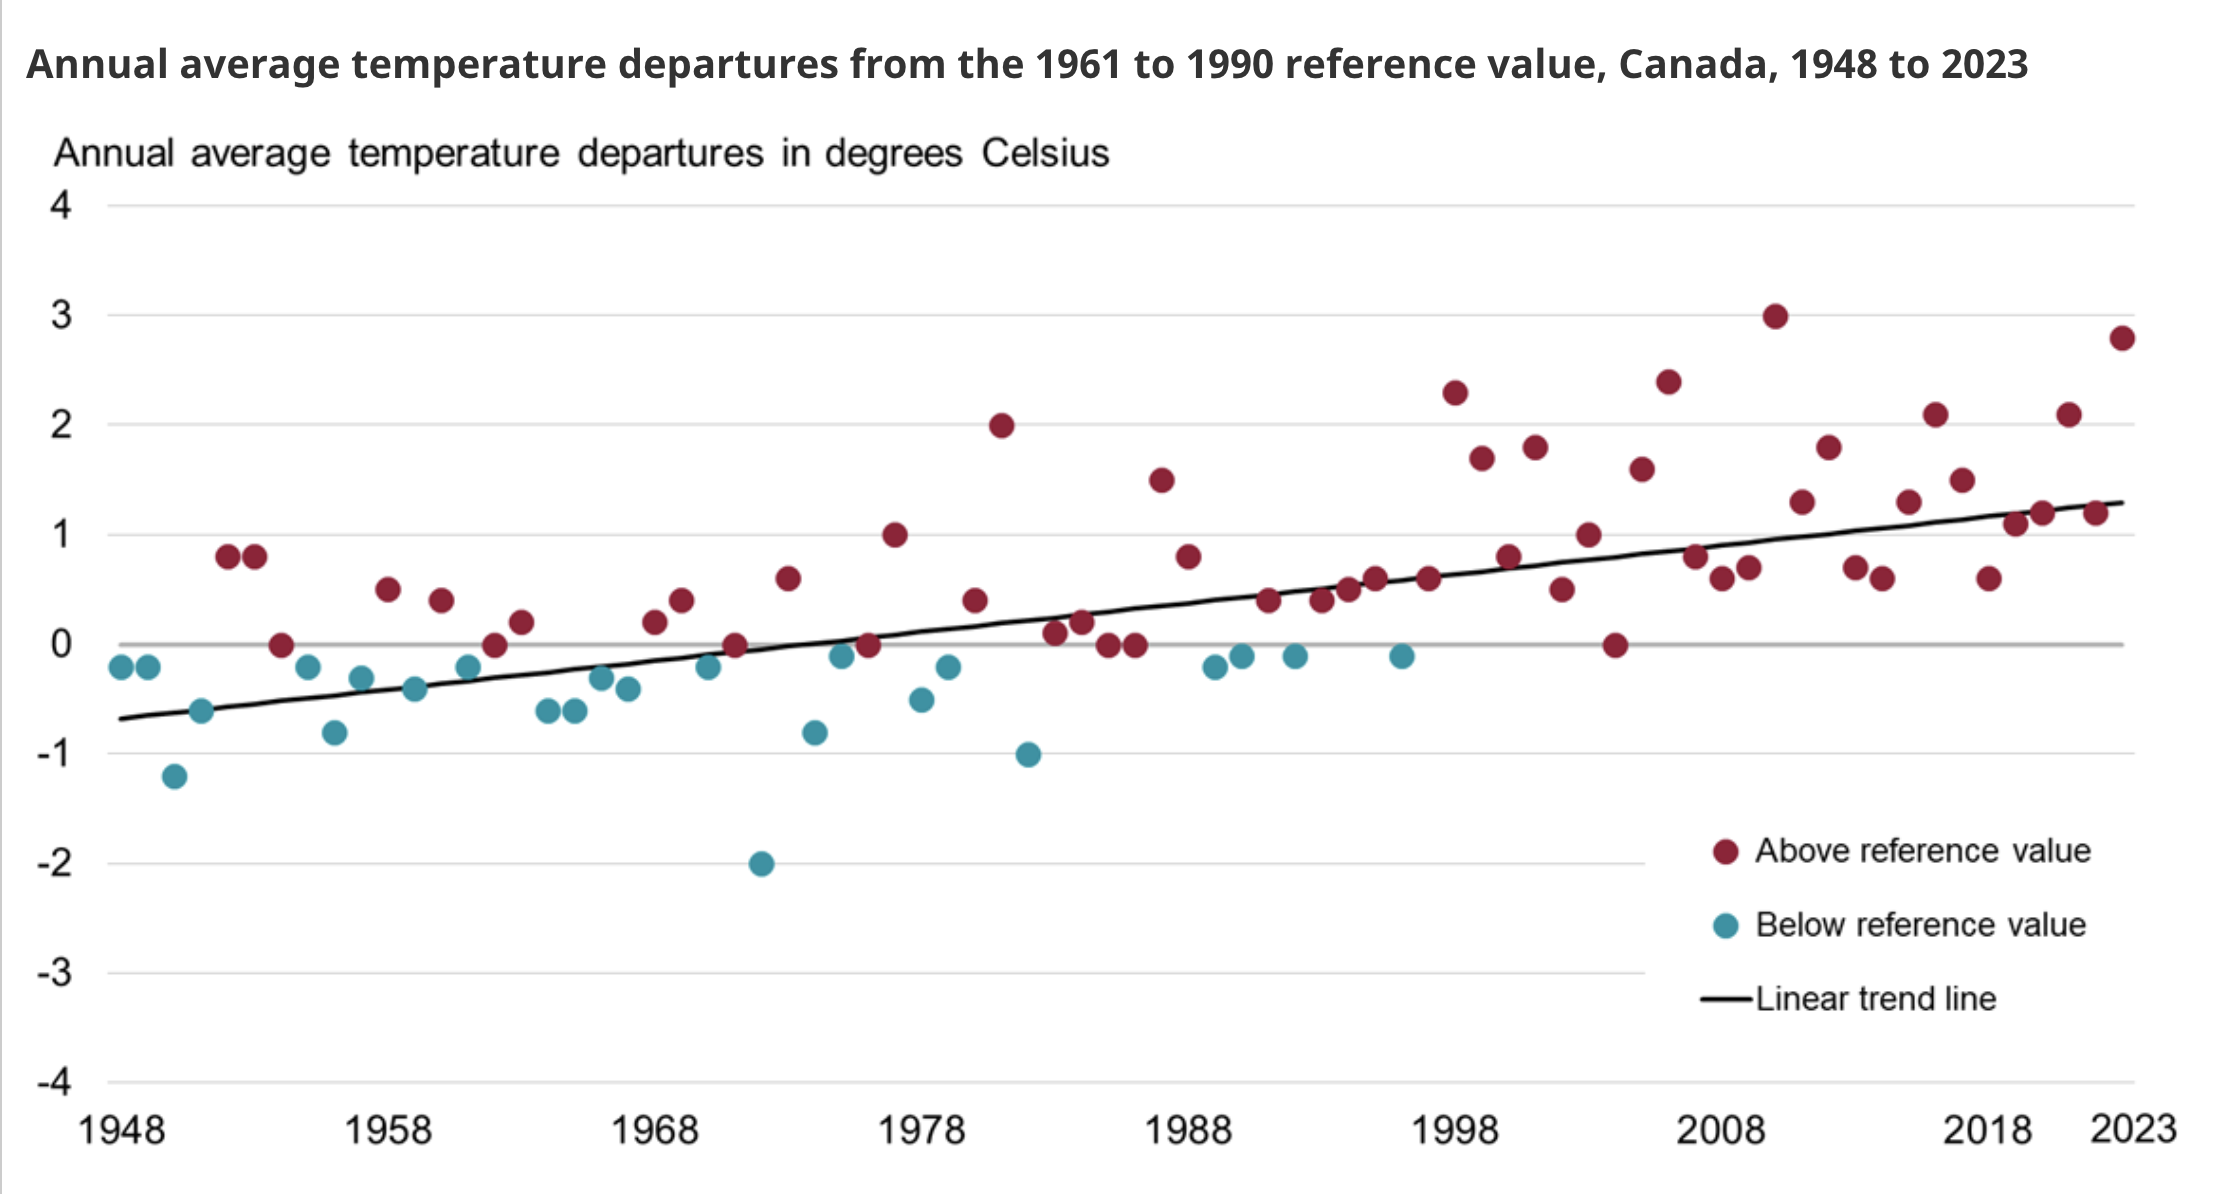
\includegraphics[scale=0.295]{Annual_temp}
      %    \includegraphics[scale=.40]{one.pdf}
      \end{center}
  \end{figure}
 \end{frame}
 
   \begin{frame} \frametitle{Why is climate change important to Canada?}
\label{Why is climate change important to Canada?}
\textbf{Canada's annual temperature change}
\begin{itemize}
\item[]
\item average temperature for the year 2023 was 2.8 degrees Celsius (\textdegree{}C) above the 1961-1990 reference value
\item[]
\begin{itemize}
\item  making it second warmest year since 1948  
\end{itemize}
\item[]

\item From 1948 to 2023, there is a trend in annual average temperature departures, showing 2.0 \textdegree{}C of warming over that period
\item[]
\item annual average temperatures were consistently above or equal to the reference value from 1997 onward
\end{itemize}

 \end{frame}
 
 
 
 \begin{frame} \frametitle{Why is climate change important to Canada?}
\label{Why is climate change important to Canada?}

\begin{figure}
    \begin{center}
      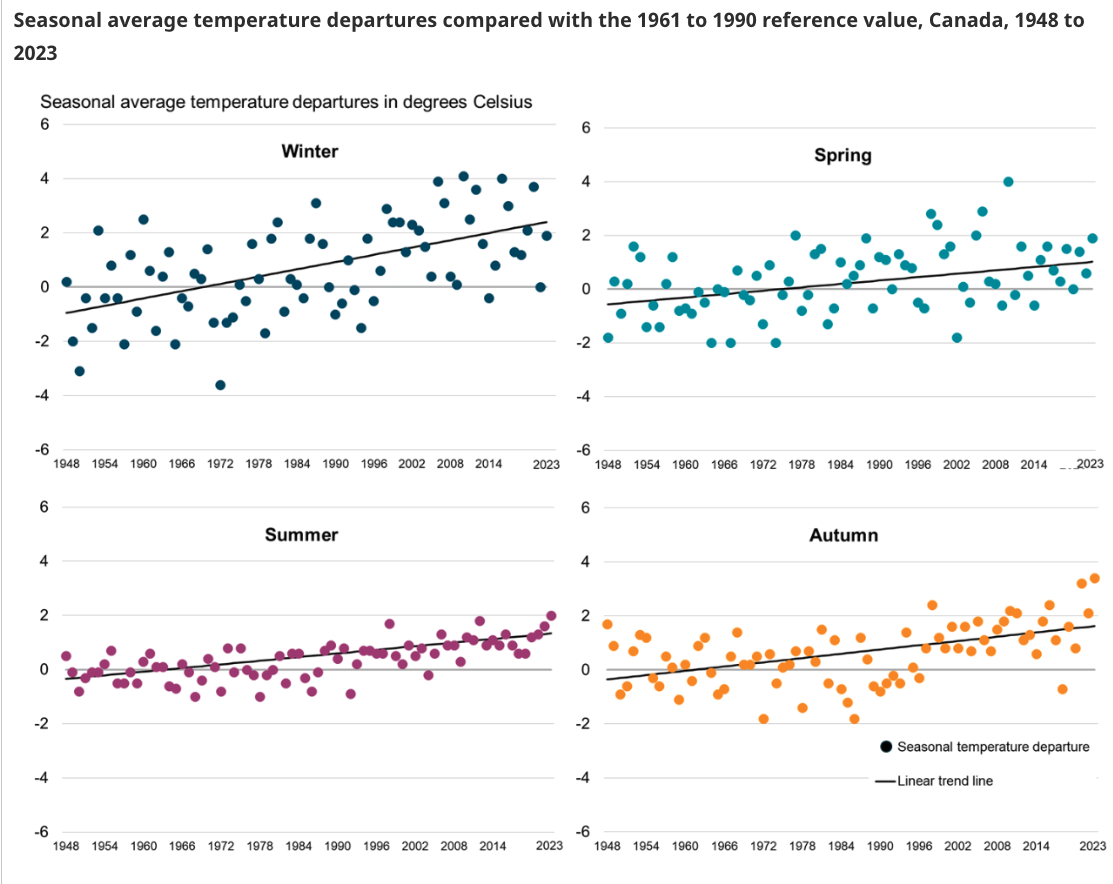
\includegraphics[scale=0.27]{Seasonal_temp}
      %    \includegraphics[scale=.40]{one.pdf}
      \end{center}
  \end{figure}
 \end{frame}
 
 
    \begin{frame} \frametitle{Why is climate change important to Canada?}
\label{Why is climate change important to Canada?}


\textbf{Canada's seasonal temperature change}
\begin{itemize}
\item[]
\item warming trends were detected for all four seasons:
\begin{itemize}
\item winter, with an increase of 3.4\textdegree{}C 
\item spring, with an increase of 1.9\textdegree{}C 
\item summer with an increase of 1.9\textdegree{}C 
\item Fall, with an increase of 2.0\textdegree{}C 
\item[]
\end{itemize}
\item the warmest winter and spring recorded were in 2010
\item[]
\item the warmest summer and fall were in 2023
\end{itemize}
 \end{frame}
 
  \begin{frame} \frametitle{Why is climate change important to Canada?}
\label{Why is climate change important to Canada?}

\begin{figure}
    \begin{center}
      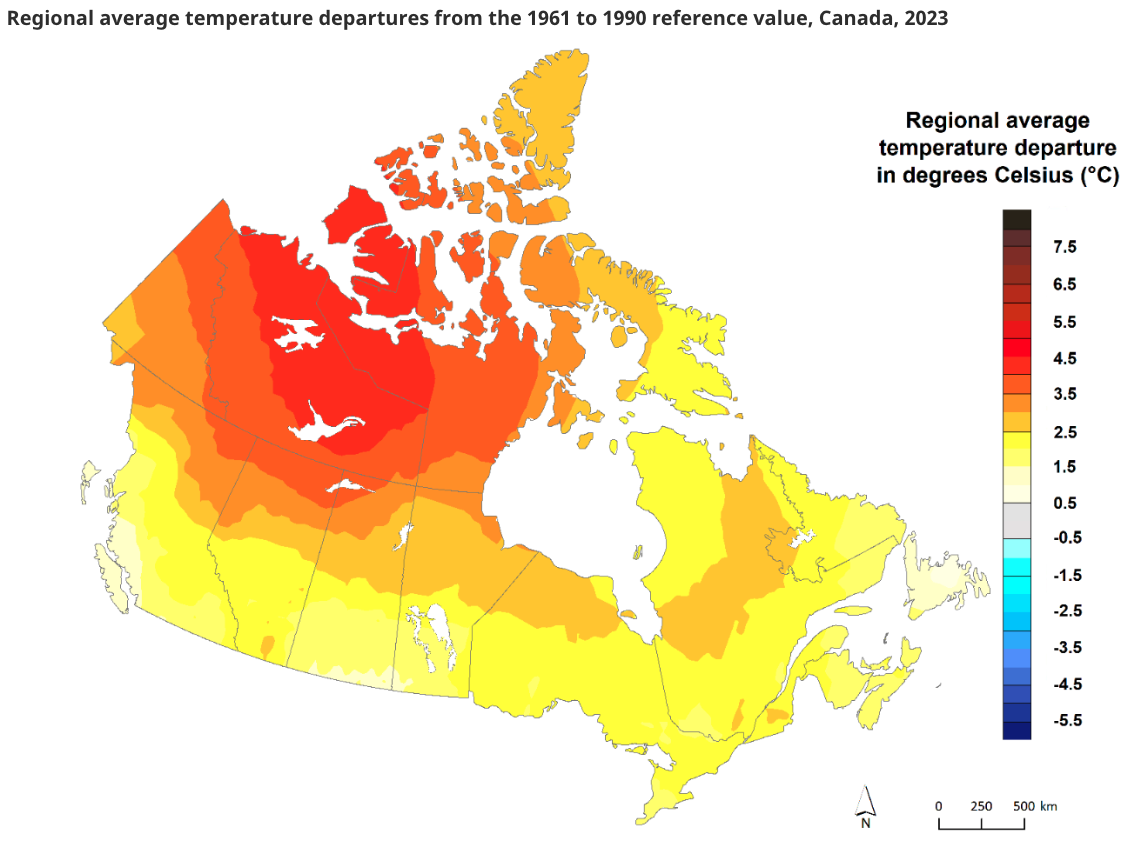
\includegraphics[scale=0.27]{Regional_temp}
      %    \includegraphics[scale=.40]{one.pdf}
      \end{center}
  \end{figure}
 \end{frame}
 
 

 
 

 
 
    \begin{frame} \frametitle{Why is climate change important to Canada?}
\label{Why is climate change important to Canada?}


\textbf{Regional temperature departures}
\begin{itemize}
\item[]
\item All regions of Canada experienced annual temperatures above the 1961-1990 reference value
\item[]
\item Most of northern Canada and the northern parts of British Columbia, the Prairies, Ontario and Quebec, experienced temperatures significantly above the baseline average
\item[]
\item Eastern Newfoundland and Labrador and western British Columbia experienced the least annual temperature departure from the baseline average


\end{itemize}
 \end{frame}
 
 
 
   \begin{frame} \frametitle{Canada's economy depends on emission-intensive sectors}
\label{Canada's economy depends on emission-intensive sectors}
\textbf{Oil and gas production accounts for the largest share of Canada's greenhouse gas emissions by economic sector (2019)}
\begin{figure}
    \begin{center}
      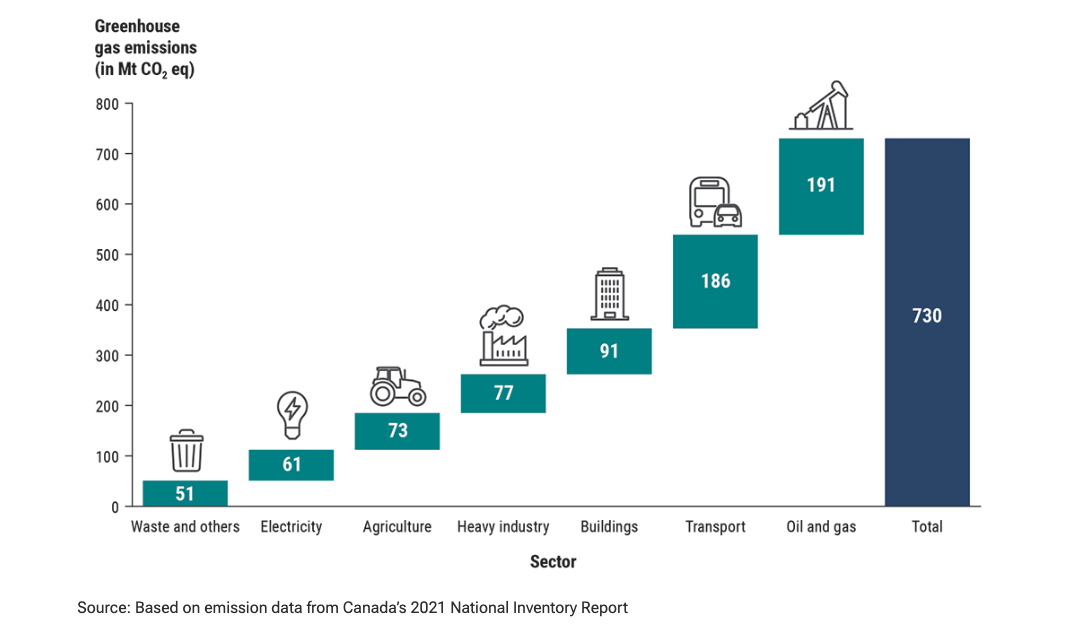
\includegraphics[scale=0.29]{sector_emission}
      %    \includegraphics[scale=.40]{one.pdf}
      \end{center}
  \end{figure}
 \end{frame}
 
 
    \begin{frame} \frametitle{Canada's economy depends on emission-intensive sectors}
\label{Canada's economy depends on emission-intensive sectors}
 In 2019,
\begin{itemize}
\item Canada emitted 730 megatonnes of carbon dioxide equivalent
\item[]
\item oil and gas production accounted for the largest share of Canada's greenhouse gas emissions by economic sector 

\end{itemize}
 \end{frame}
 
 
 
    \begin{frame} \frametitle{Comparing Canada's GHG emissions to global levels}
\label{GHG comparison}

\begin{figure}
    \begin{center}
      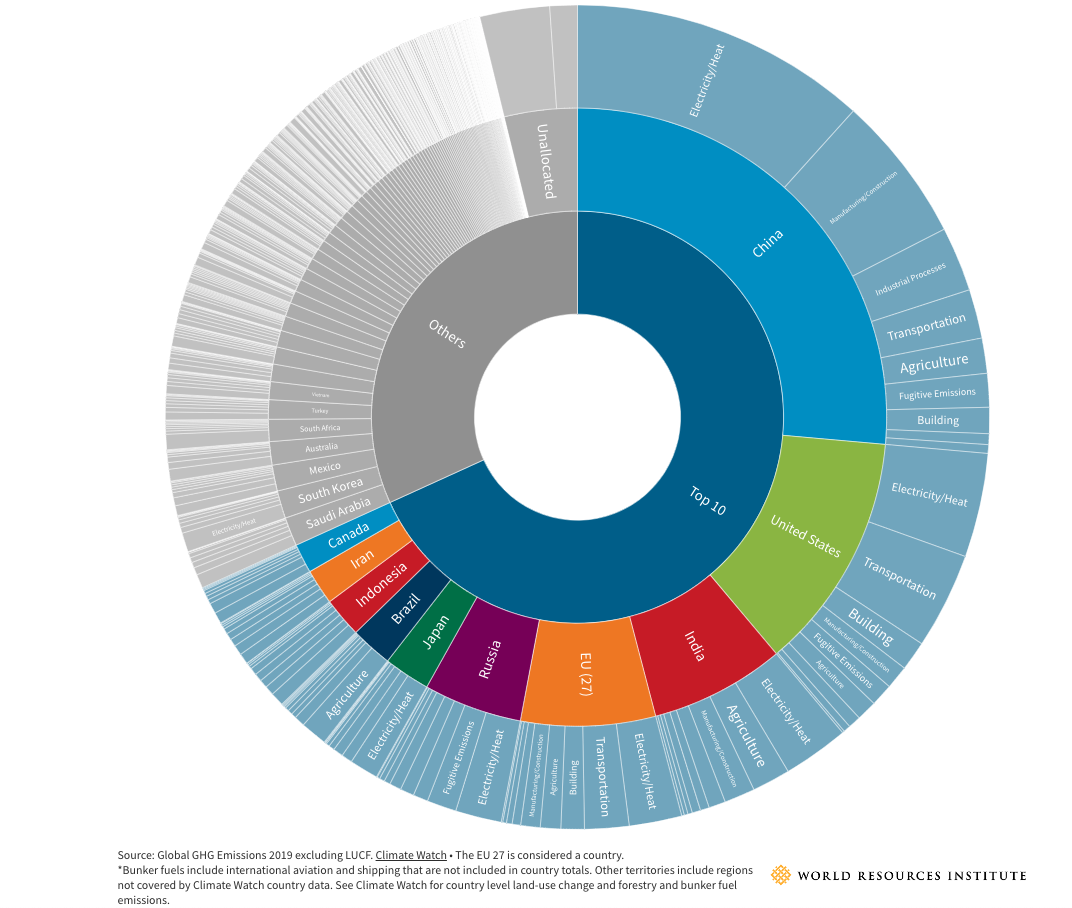
\includegraphics[scale=0.23]{ghg_world}
      %    \includegraphics[scale=.40]{one.pdf}
      \end{center}
  \end{figure}
 \end{frame}
 
 
 
     \begin{frame} \frametitle{Comparing Canada's GHG emissions to global levels}
\label{GHG comparison}
\begin{itemize}
\item China is the biggest emitter $\rightarrow 26.4\%$ of global greenhouse gas emissions
\item[]
\item United States $\rightarrow 12.5\%$
\item[]
\item India $\rightarrow 7.06\%$
\item[]
\item European Union $\rightarrow 7.03\%$
\item[]
\end{itemize}

Canada contributes approximately $1.5\%$ of the global GHG emissions.
 \end{frame}
 
 
 
 
      \begin{frame} \frametitle{The Economics of Climate Change}
\label{The Economics of Climate Change}
\textbf{Externalities and Market Failures:}
\begin{itemize}
\item[]
\item \textbf{Negative Externalities:} climate change is a classic negative externality, where the social costs of emissions are not reflected in market prices
\item[]
\item Carbon emissions from transportation, energy production, and industry impose costs on society, including:

\begin{itemize}

\item \textbf{health costs} due to air pollution
\item \textbf{Environmental damage} like rising sea levels and more frequent extreme weather events
\item \textbf{Economics losses} in sectors like agriculture, tourism, and infrastructure
\end{itemize}

\end{itemize}
\textbf{Example:}
\begin{itemize}
\item Canada's oil sands present a case of over-reliance on carbon-intensive energy, where the social cost of pollution is externalized

\end{itemize}
 \end{frame}
 
 
 
       \begin{frame} \frametitle{The Economics of Climate Change}
\label{The Economics of Climate Change}
\textbf{Public Goods:}
\begin{itemize}

\item non-excludable and non-rivalrous resources from which everyone benefits
\item[]
\item examples: clean air, stable climates, and healthy ecosystems
\item[]
\item since no one can be excluded from enjoying a stable climate, there is little incentive for individual actors (countries, companies, or individuals) to voluntarily reduce emissions, leading to the \textbf{free rider problem}
\item[]
\item Canada,  contributing only $1.5\%$ of global emissions, is susceptible to the global free-rider problem, depending on international cooperation to combat climate change

\end{itemize}
 \end{frame}
 
 
 
        \begin{frame} \frametitle{Policy Responses to Climate Change: Carbon Pricing as a Market-Based Solution}
\label{Policy Responses to Climate Change: Carbon Pricing as a Market-Based Solution}
\textbf{Pigovian Taxes:}
\begin{itemize}
\item carbon taxes are an example of Pigovian taxes

\item designed to correct a negative externality by making polluters pay the social cost of their emissions

\item by internalizing the cost of carbon, carbon pricing aligns private costs with social costs
\item[]
\end{itemize}

\textbf{Canada's national carbon pricing policy:}

\begin{itemize}
\item implemented in 2019
\item is a model for a Pigovian tax in action
\item targeting carbon price of $CAD \$170$ per tonne by 2030
\item encourages reductions in emissions by making carbon-intensive goods and services more expensive
\end{itemize}
 \end{frame}
 
 
         \begin{frame} \frametitle{Policy Responses to Climate Change: Carbon Pricing as a Market-Based Solution}
\label{Policy Responses to Climate Change: Carbon Pricing as a Market-Based Solution}


\textbf{British Columbia's Carbon Tax:}

\begin{itemize}
\item introduced in 2008
\item starting at  $CAD \$10$ per tonne of CO2 and gradually increasing
\item led to a significant reduction in emissions without harming the economy
\item proving the effectiveness of Pigovian taxes in correcting market failures
\end{itemize}
 \end{frame}
 
 
 
     \begin{frame} \frametitle{Carbon Tax}
\label{GHG comparison}

\begin{figure}
    \begin{center}
      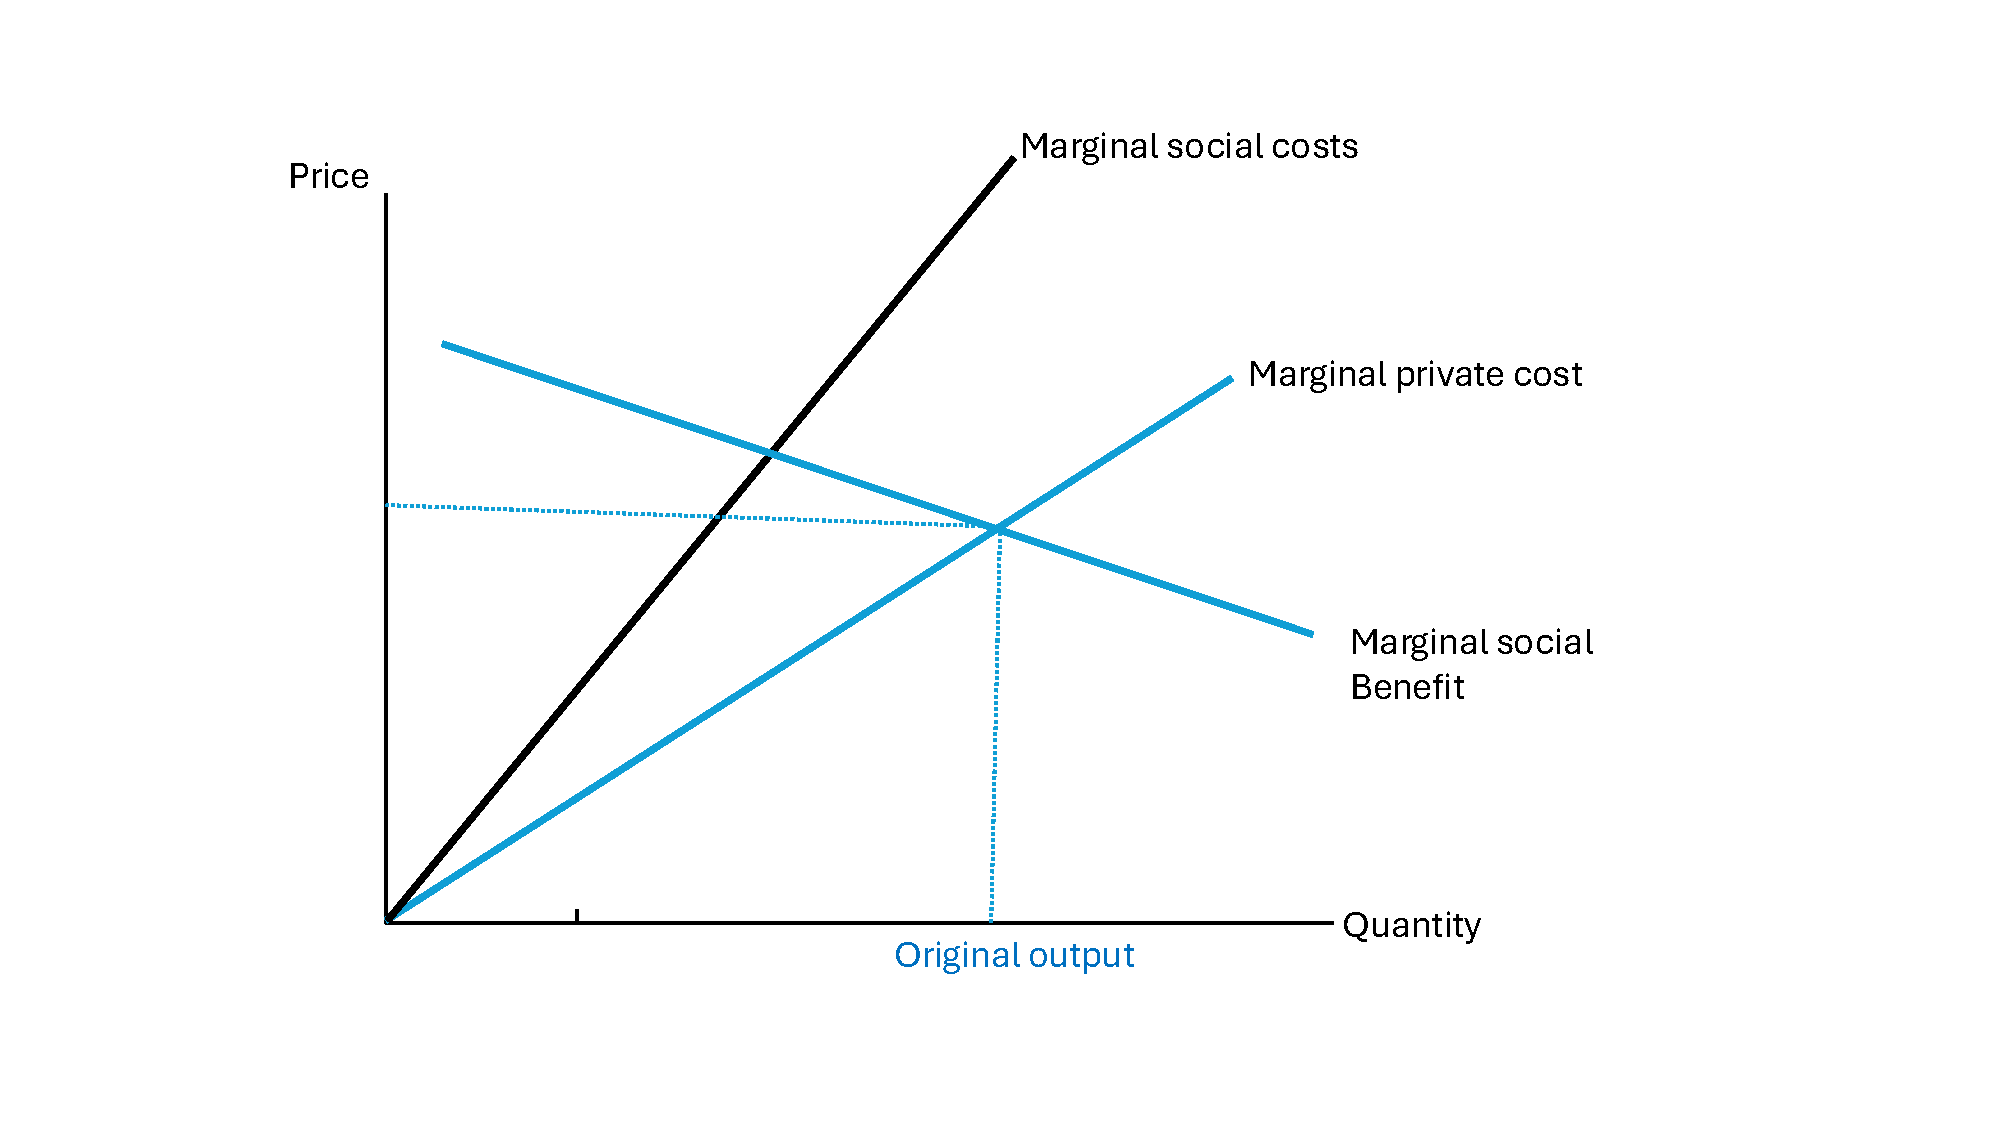
\includegraphics[scale=0.4]{Pigovian1a}
      %    \includegraphics[scale=.40]{one.pdf}
      \end{center}
  \end{figure}
 \end{frame}
 
 
      \begin{frame} \frametitle{Carbon Tax}
\label{GHG comparison}

\begin{figure}
    \begin{center}
      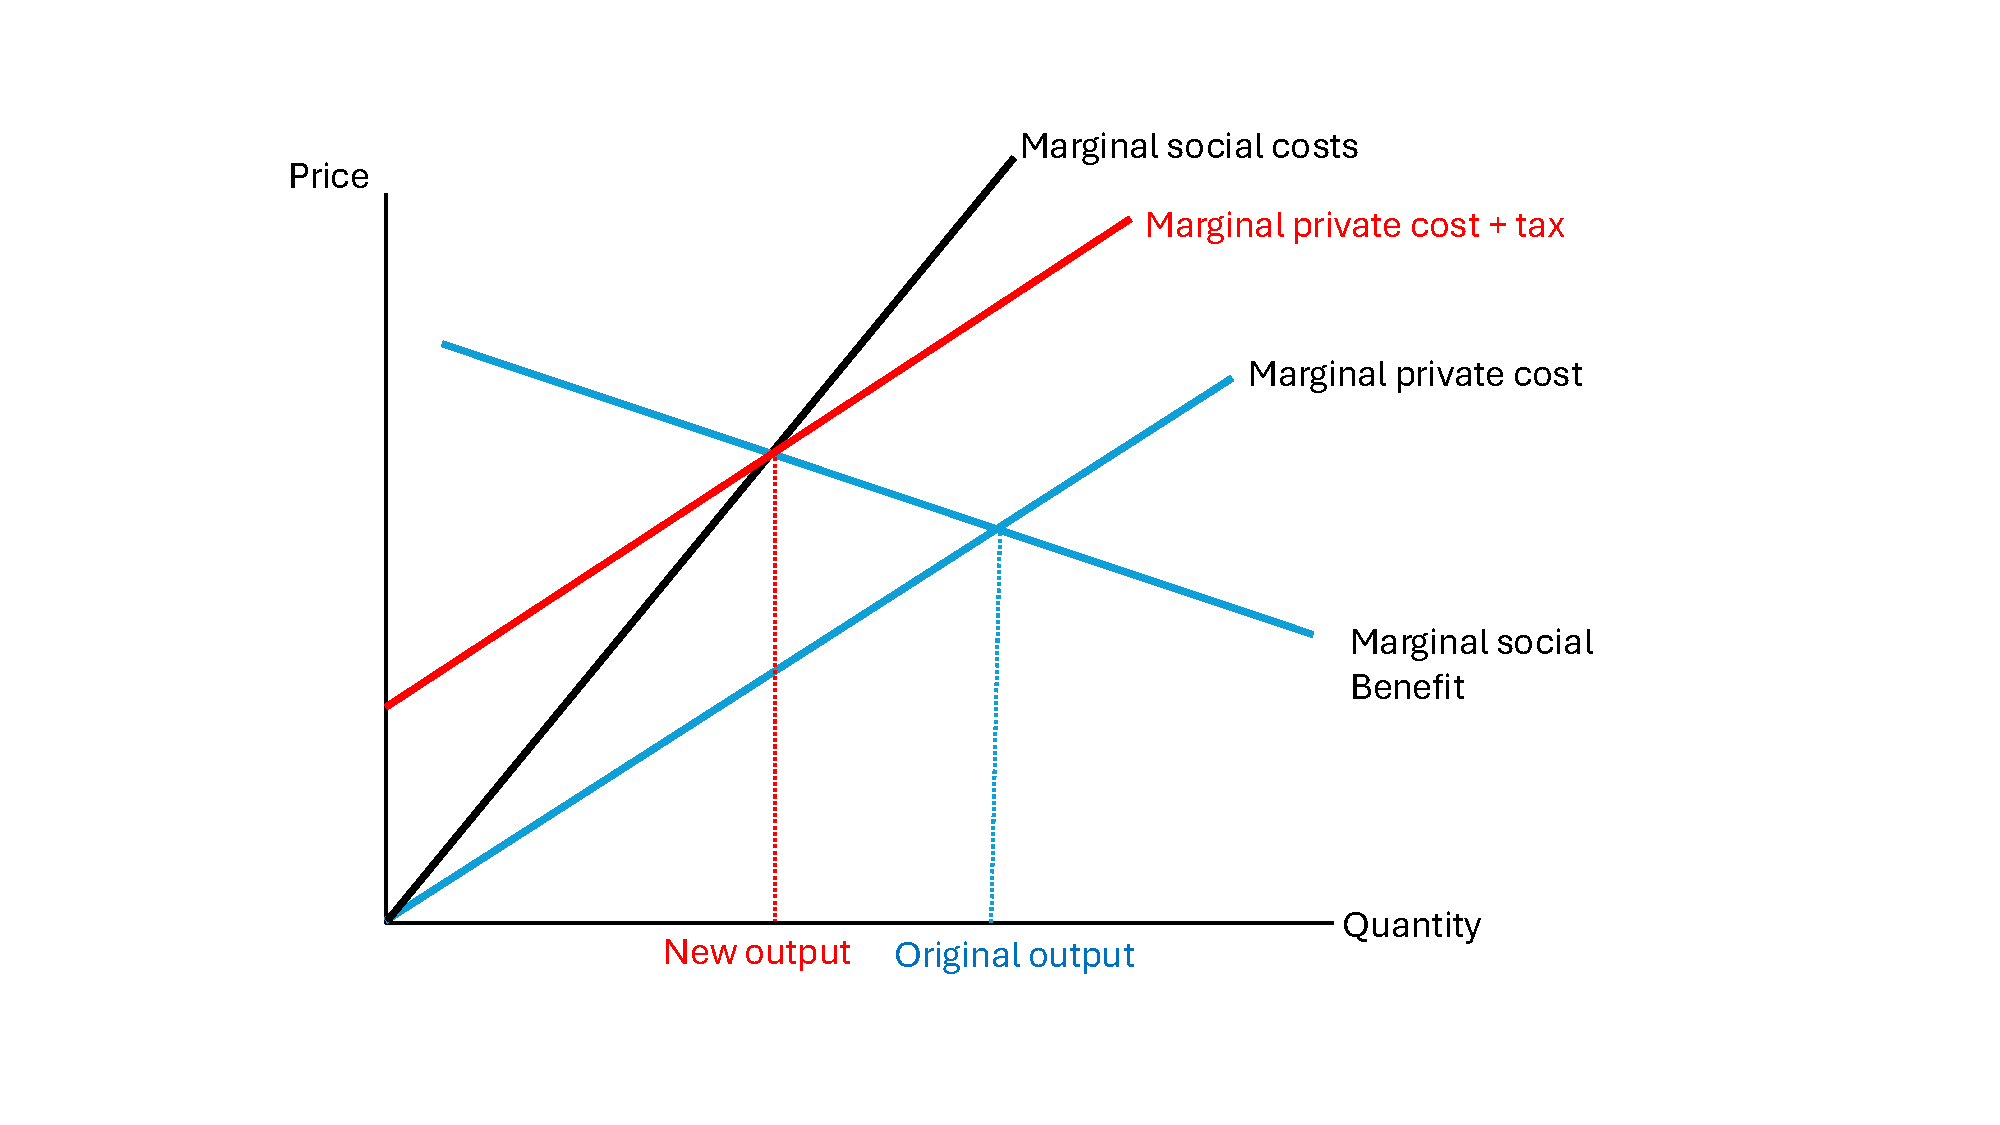
\includegraphics[scale=0.4]{Pigovian1b}
      %    \includegraphics[scale=.40]{one.pdf}
      \end{center}
  \end{figure}
 \end{frame}
 
      \begin{frame} \frametitle{Carbon Tax}
\label{GHG comparison}

\begin{figure}
    \begin{center}
      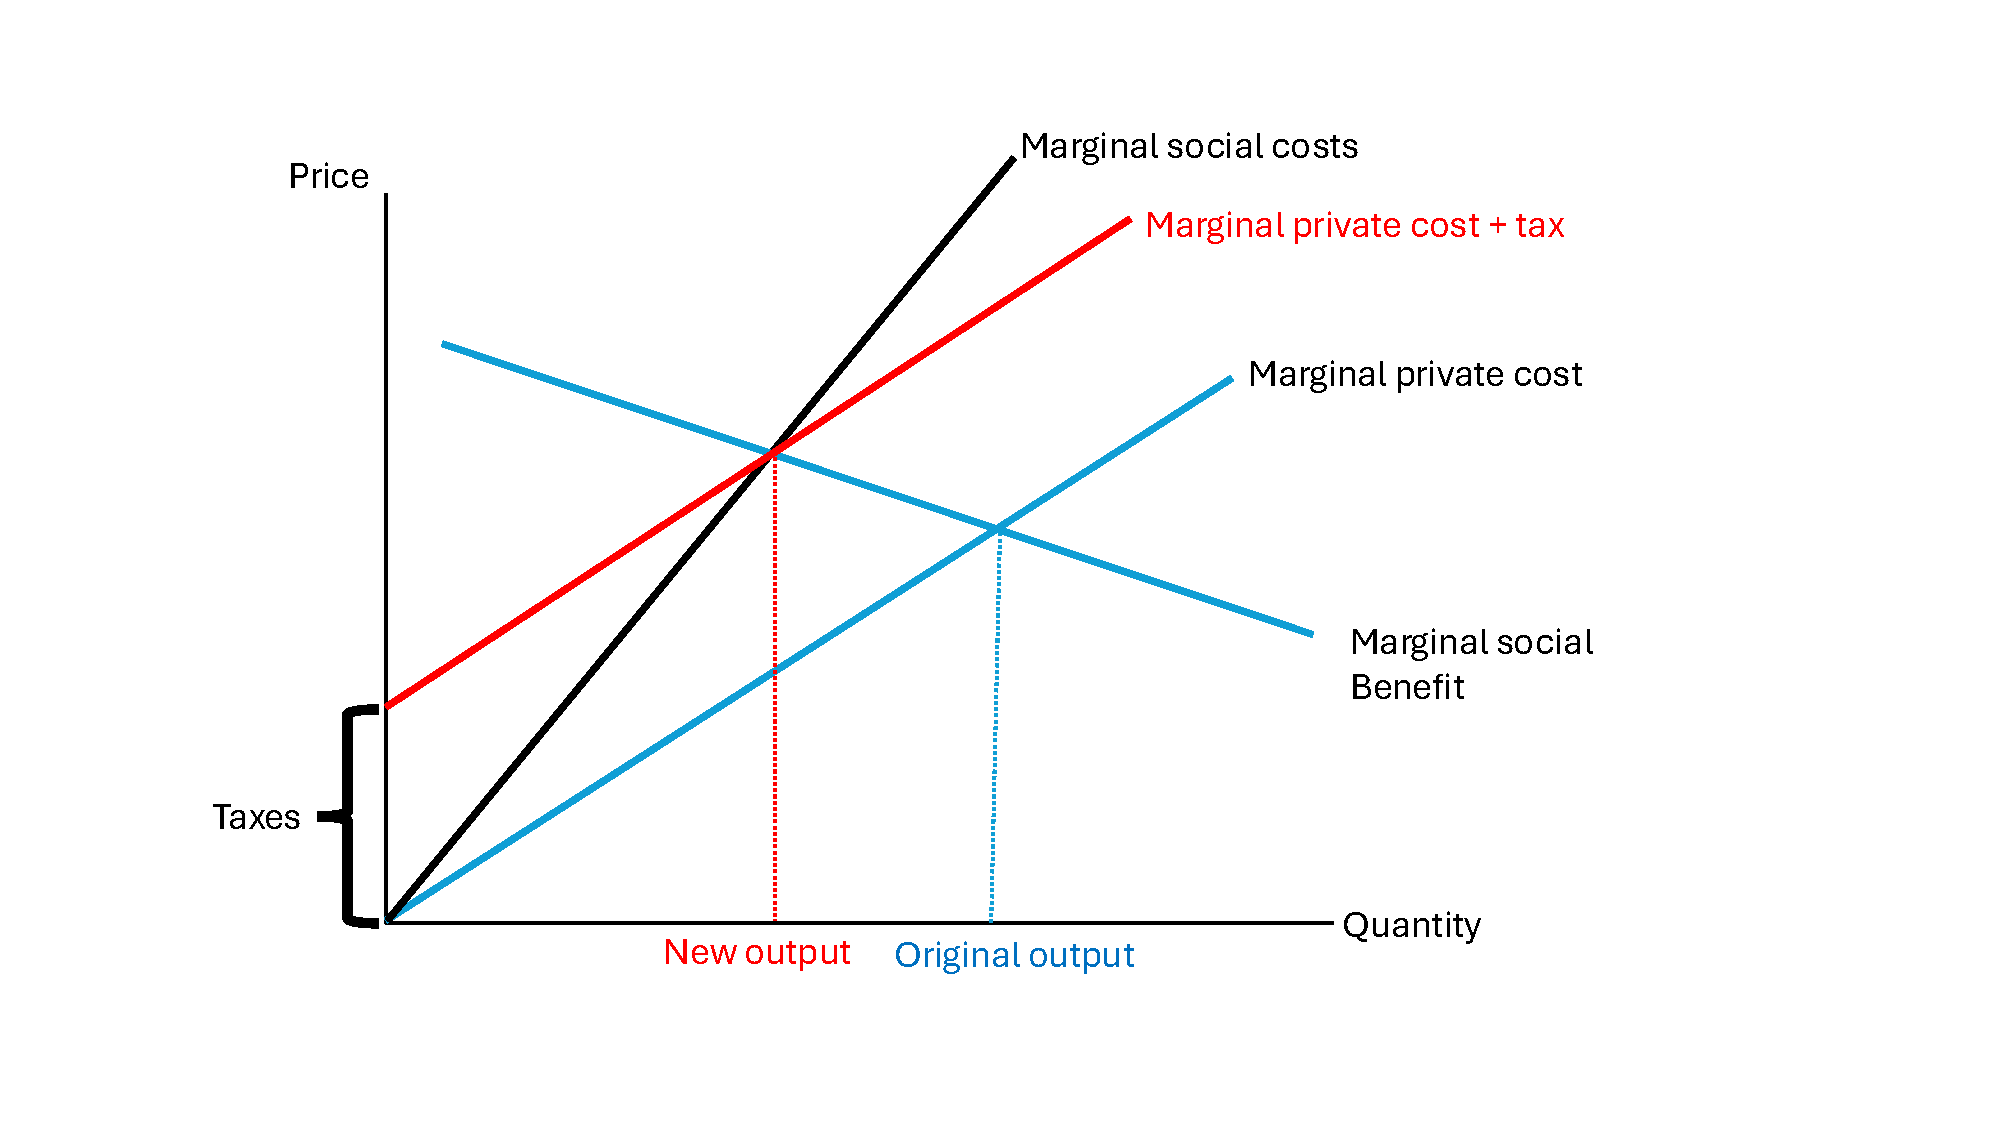
\includegraphics[scale=0.4]{Pigovian1c}
      %    \includegraphics[scale=.40]{one.pdf}
      \end{center}
  \end{figure}
 \end{frame}
 
 
       \begin{frame} \frametitle{Carbon Tax}
\label{GHG comparison}

\begin{figure}
    \begin{center}
      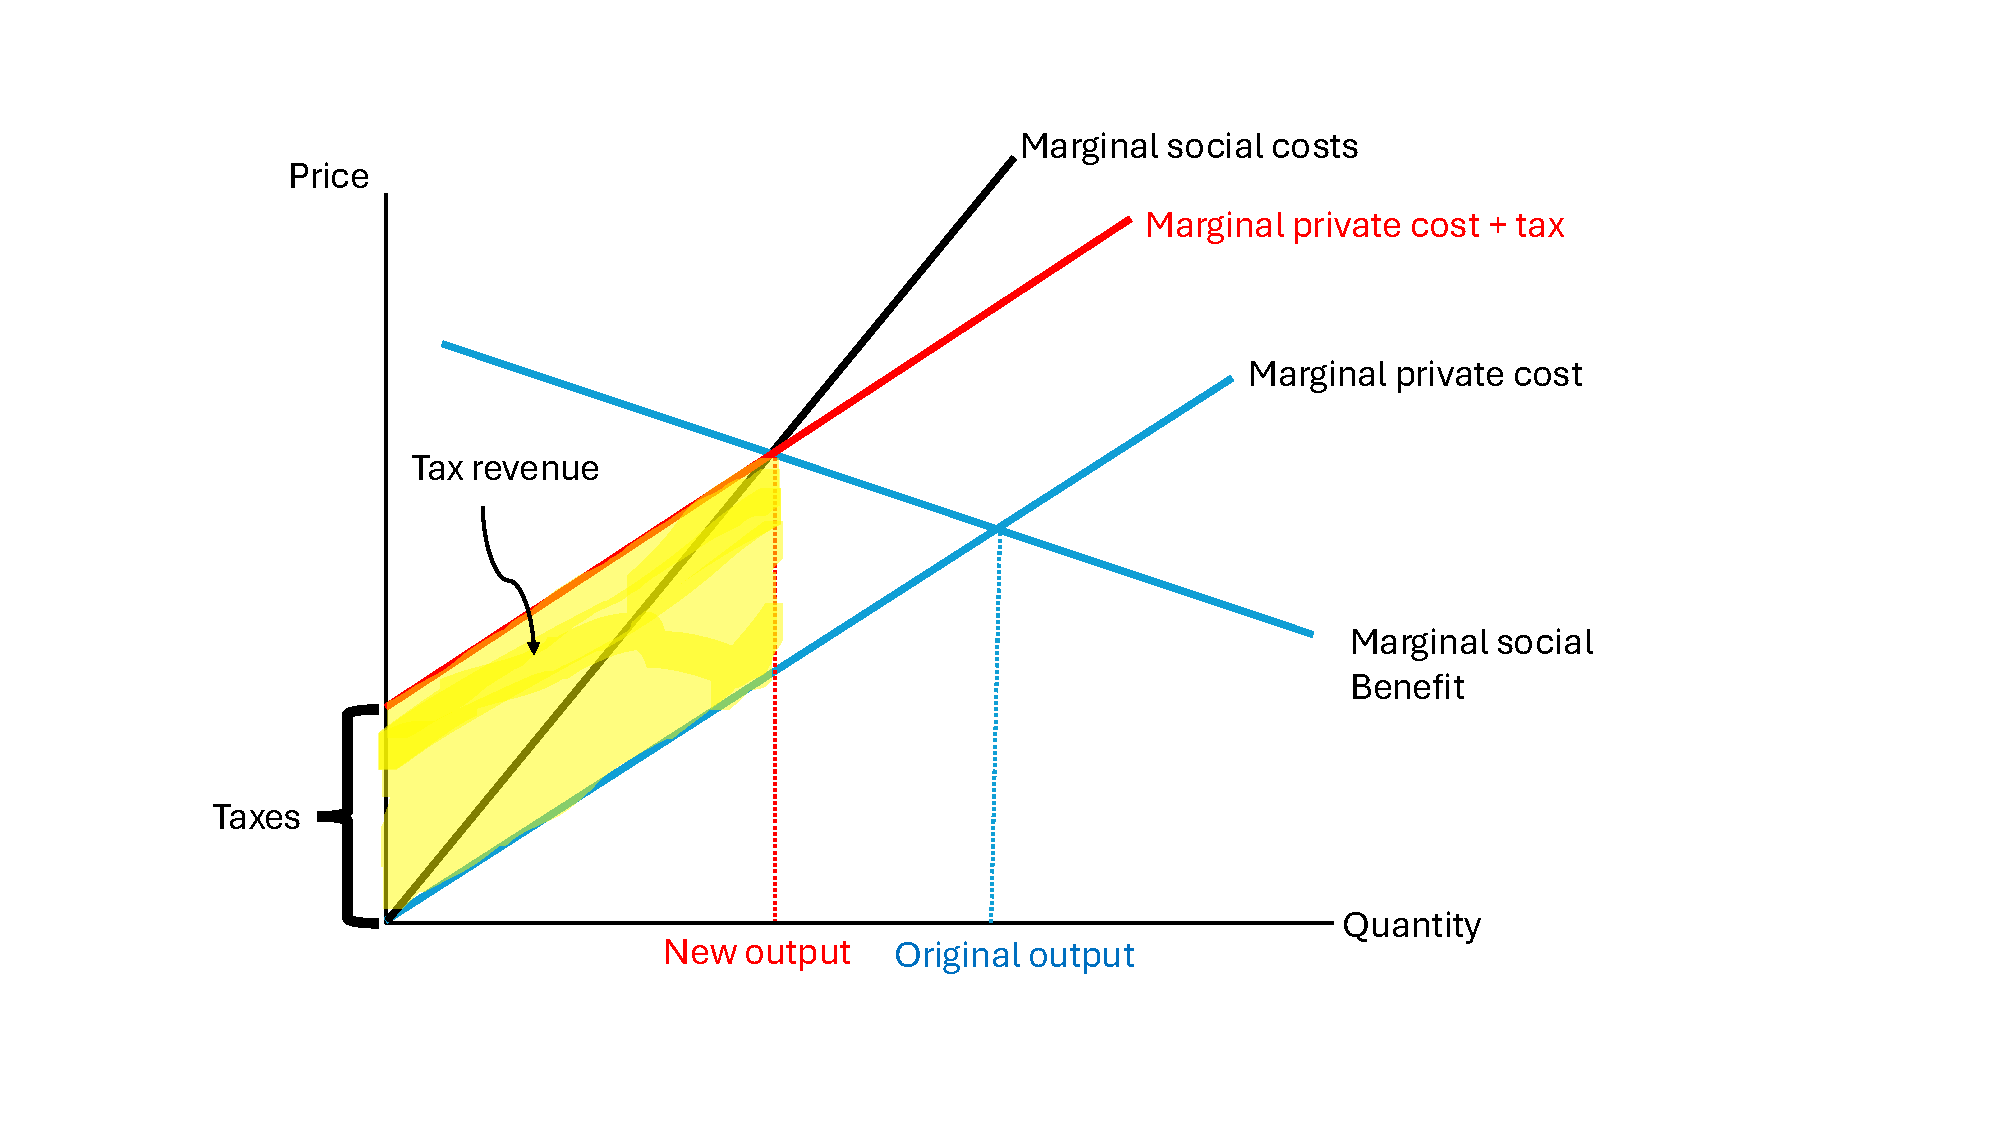
\includegraphics[scale=0.4]{Pigovian1d}
      %    \includegraphics[scale=.40]{one.pdf}
      \end{center}
  \end{figure}
 \end{frame}
 

      \begin{frame} \frametitle{Carbon Tax}
\label{GHG comparison}

\begin{itemize}
\item carbon tax is intended to correct a negative externality (e.g.,  GHG emission)
\item[]
 \item the tax is set equal to the marginal external cost of the negative externality, meaning the additional harm each unit of production or consumption imposes on society
 \item[]
\item the socially optimal output occurs where marginal social cost equals marginal social benefit
\item[]
\item the marginal social cost reflects the sum of marginal private cost and marginal external cost 
\item[]
\item the carbon tax internalizes the external cost, shifting the supply curve to match the marginal social cost curve

\end{itemize}
 \end{frame}




      \begin{frame} \frametitle{Carbon Tax}
\label{GHG comparison}

\begin{itemize}

\item when the carbon tax is applied, it raises the price to reflect the true social cost of each unit
\item[]
\item at the socially optimal quantity, the price consumers pay equals the marginal benefit of the good, which also matches the marginal social cost
\item[]
\item with carbon tax, the market equilibrium aligns with the point where price = marginal benefit = marginal social cost
\item[]
\item this condition corrects the market failure by ensuring the quantity produced is optimal from society's perspective
\end{itemize}
 \end{frame}


      \begin{frame} \frametitle{Carbon Tax Rate in Canada}
\label{GHG comparison}

\begin{itemize}
\item Canada's federal carbon tax is $\$ 80$ per tonne of carbon dioxide equivalent ($CO_{2}e$)
\item[]
\item this tax applies to fossil fuels such as gasoline, diesel, natural gas, and heating oil
\item[]
\item the scheduled rates are as follows:
\begin{itemize}
\item 2019: $\$ 20$ per tonne $CO_{2}e$
\item 2020: $\$ 30$ per tonne $CO_{2}e$
\item 2021: $\$ 40$ per tonne $CO_{2}e$
\item 2022: $\$ 50$ per tonne $CO_{2}e$
\item 2023: $\$ 65$ per tonne $CO_{2}e$
\item 2024: $\$ 80$ per tonne $CO_{2}e$

\end{itemize}
\item[]
\end{itemize}
The Canadian government has outlined plans to continue increasing the carbon tax by  $\$15$ per tonne annually, aiming to reach  $\$170$ per tonne $CO_{2}e$ by 2030.
 \end{frame}







      \begin{frame} \frametitle{Question:}
\label{GHG comparison}


How does the government use the revenue collected from the carbon tax?
 \end{frame}


      \begin{frame} \frametitle{Answer:}
\label{GHG comparison}
\begin{itemize}


\item approximately $90\%$ of the revenue is returned to individuals through the Canada Carbon Rebate
\item[]
\item the remaining $10\%$ goes back to farmers,  small-and medium-enterprises and Indigenous governments
\end{itemize}
 \end{frame}



      \begin{frame} \frametitle{Climate Change and Sustainability}
\label{GHG comparison}

Carbon tax is considered a component of sustainability as it aligns economic incentives with environmental goals by promoting reduced greenhouse gas emissions and encouraging clean energy adoption\\


\textbf{How does it fit sustainability?}
\begin{itemize}


\item \textbf{Environmental Protection:} The carbon tax discourages the use of fossil fuels by making carbon emissions costly.  By putting a price on carbon, it helps lower pollution levels and mitigate climate change, directly supporting environmental sustainability
\item[]
\item \textbf{Resource Efficiency:} Carbon taxes encourage more efficient use of resources by motivating businesses and individuals to adopt energy-efficient practices and technologies
\end{itemize}
 \end{frame}



      \begin{frame} \frametitle{Climate Change and Sustainability cont'd}
\label{GHG comparison}

\begin{itemize}


\item \textbf{Economic Sustainability:} Revenue from carbon taxes can be invested in renewable energy projects, energy-efficient infrastructure, and public rebates, which contribute to economic resilience and a green transition
\item[]
\item \textbf{Social Equity:} When combined with measures like rebates (e.g., Canada's Carbon Rebate), carbon taxes can be structured to protect low- and middle-income households from financial burdens, supporting social sustainability by ensuring fair distribution of costs
\item[]
\end{itemize}
Therefore,  a carbon tax is a policy tool that supports sustainability by addressing economic, environmental, and social dimensions in the effort to combat climate change
 \end{frame}

     \begin{frame} \frametitle{Case Studies - In-Class Group Exercise}
\label{GHG comparison}

Form groups of 3-4 students and select one of the following case studies to research and discuss with your group members.

\begin{enumerate}
\item[]
\item British Columbia's Carbon Tax
\item Ontario's Green Energy Act (GEA)
\item Alberta's Oil Sands and Climate Initiatives
\item Indigenous-Led Conservation in the Great Bear Rainforest
\end{enumerate}

 \end{frame}

      \begin{frame} \frametitle{Critical Thinking Question:}
\label{GHG comparison}

Given Canada's commitment to increasing the carbon tax to $\$ 170$ per tonne by 2030, evaluate the potential economic and social impacts of this policy on different sectors (e.g., households, businesses, and energy-intensive industries). Consider both positive and negative effects. Do you think the revenue-recycling strategy through rebates is effective in addressing these impacts, or should additional measures be taken to ensure fairness and effectiveness in achieving Canada's climate goals?

 \end{frame}




     \begin{frame} \frametitle{Answer to Critical Thinking Question:}
\label{GHG comparison}

\textbf{Will be discussed during next Lecture}

 \end{frame}








 \begin{frame} \frametitle{References}
\label{References}
\begin{itemize}
 \item Climate Watch Historical GHG Emissions. 2022. Washington, DC: World Resources Institute. Available online at: https://www.climatewatchdata.org/ghg-emissions
 \item[]
 \item Environment and Climate Change Canada (2024) Canadian Environmental Sustainability Indicators: Temperature change in Canada. Consulted on Month day, year.  Available at: www.canada.ca/en/environment-climate-change/services/environmental-indicators/temperaturechange.html. 
 \item[]

 \item How carbon pricing works. Available at: https://www.canada.ca/en/environment-climate-change/services/climate-change/pricing-pollution-how-it-will-work/putting-price-on-carbon-pollution.html
 

 
\end{itemize}
 \end{frame}


 \begin{frame} \frametitle{References cont'd}
\label{References}
\begin{itemize}
 \item Lessons Learned from Canada's Record on Climate Change.  Available at: https://www.oag-bvg.gc.ca
 \item[]
\item Lulham, N., Warren, F.J., Walsh, K.A. and Szwarc, J. (2023). Canada in a Changing Climate: Synthesis Report; Government of Canada, Ottawa, Ontario.
\item[]
\item Parkin, M.,  $\&$ Bade, R. (2020). Microeconomics (12th ed.). Pearson.
\item[]
\item Reed, G., Fox, S., Littlechild, D., McGregor, D., Lewis, D., Popp, J., Wray, K., Kassi, N., Ruben, R., Morales, S. and Lonsdale, S. (2024). For Our Future: Indigenous Resilience Report. Ottawa, Ontario.
\item[]

\end{itemize}
 \end{frame}

\end{document}
